% =============================================================================
% PART B - MODULE 2: AUTHENTICATION & SESSION MANAGEMENT (M2.01 - M2.07)
% In Charge: Nguyen Tien Thuan (CE181024)
% =============================================================================

\section{User Manual}

\subsection{Overview of the Application \& System Actors}

\textbf{Frevia} is an enterprise-grade, \textbf{AI-Powered Freelance Marketplace and Professional Community Platform} engineered to bridge businesses and elite freelance professionals through automated talent matching, milestone-governed escrow smart contracts, and real-time collaboration tools. Built on a resilient \textbf{Role-Based Access Control (RBAC)} architecture, system capabilities and operational permissions are distributed across five primary actor groups:

\begin{itemize}[leftmargin=1.5em,itemsep=3pt]
  \item \textbf{Guest (Unauthenticated Visitor):} Explores public job postings, reviews top-rated freelancer and expert portfolios, browses open community discussions, and executes self-service onboarding or sign-in flows.
  \item \textbf{Freelancer (Independent Talent):} Curates comprehensive multi-faceted profiles, uploads resumes for AI parsing, completes eKYC identity verification, submits bids on posted jobs, negotiates milestone contracts, submits deliverables, and receives payments via Stripe Connect.
  \item \textbf{Client (Employer / Enterprise Buyer):} Manages organization profiles, authors detailed job requisitions, evaluates incoming freelancer proposals, enters into binding milestone contracts, deposits escrow funds, approves deliverables, and submits ratings.
  \item \textbf{Expert (Specialist Consultant):} Operates within an exclusive consultation workspace (\texttt{/expert/profile}), submits credentials for administrative revision approvals, and delivers high-tier advisory services.
  \item \textbf{Administrator (System Governor):} Exercises unrestricted governance across the dedicated \texttt{/admin} portal: orchestrating dynamic RBAC role-permission assignments, administering multi-profile user directories, maintaining system-wide master catalogs (Skills, Job Categories, Forum Categories), moderating community content, approving eKYC submissions, and mediating milestone dispute arbitrations.
\end{itemize}

\newpage
% =============================================================================
\subsection{Module 2: Authentication \& Session Management}

The Authentication and Session Management module delivers defense-in-depth security infrastructure, featuring: 6-digit email OTP verification, \texttt{bcrypt} salted password hashing, stateless \texttt{AccessToken} and stateful \texttt{RefreshToken} pairs stored in hardened \texttt{HttpOnly} cookies, seamless \textbf{Google OAuth 2.0} single sign-on, self-service password recovery, and multi-device active session auditing with remote revocation capabilities.

% -----------------------------------------------------------------------------
\subsubsection{M2.01 -- New User Registration \& Email OTP Verification (UC-01)}

\begin{itemize}[leftmargin=1.5em,itemsep=2pt]
  \item \textbf{Screen Name \& Route Path:} User Registration Screen -- \texttt{/register}.
  \item \textbf{Target Actor:} Guest (New visitor without an existing account).
  \item \textbf{Preconditions:} The user is not currently authenticated and possesses an accessible email address not previously registered on Frevia.
\end{itemize}

\begin{figure}[H]
  \centering
  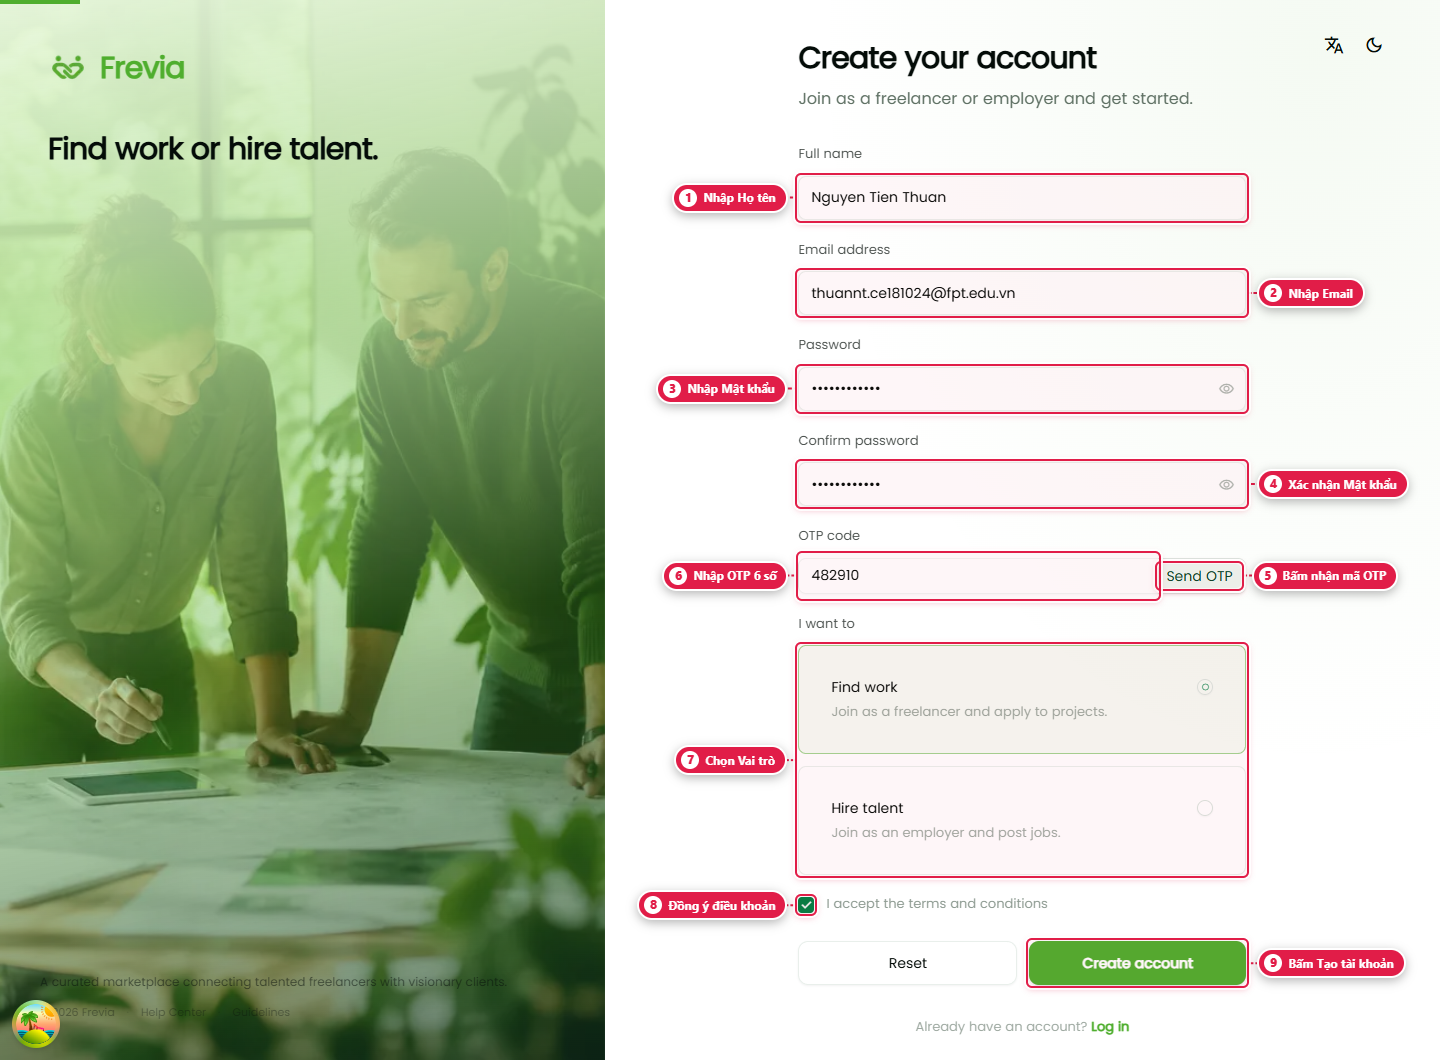
\includegraphics[width=0.90\textwidth]{images/auth/m02_01_register.png}
  \caption{User Registration and Email OTP Verification interface at \texttt{/register}}
\end{figure}

\paragraph{Step-by-Step User Instructions:}
\begin{enumerate}[leftmargin=1.8em,itemsep=3pt]
  \item \rbadge{1} \textbf{Enter Full Name (\textit{Full name}):} Type the legal or professional full name into the \textit{Full name} field (maximum 100 characters, e.g., \texttt{Nguyen Tien Thuan}).
  \item \rbadge{2} \textbf{Enter Email Address (\textit{Email address}):} Type a valid personal or business email address into the \textit{Email address} field.
  \item \rbadge{3} \textbf{Enter Password (\textit{Password}):} Type a strong password (minimum 6 characters). Users may click the eye icon on the right to toggle password visibility.
  \item \rbadge{4} \textbf{Confirm Password (\textit{Confirm password}):} Retype the exact password entered in step 3 to prevent typographical errors.
  \item \rbadge{5} \textbf{Request Verification OTP (\textit{Send OTP}):} Click the blue \textbf{Send OTP} button adjacent to the OTP field. The server generates a cryptographic 6-digit code, caches it in Redis with a 5-minute time-to-live (TTL), dispatches it via Gmail SMTP, and activates a 60-second cooldown timer.
  \item \rbadge{6} \textbf{Enter Verification OTP (\textit{OTP code}):} Inspect the email inbox, copy the 6-digit verification code, and enter it into the \textit{OTP code} field.
  \item \rbadge{7} \textbf{Select Account Intention (\textit{I want to}):} Choose an initial operational role:
    \begin{itemize}
      \item \textbf{Find work (Freelancer):} Register as a service provider to build a portfolio and submit job proposals.
      \item \textbf{Hire talent (Client):} Register as an enterprise or individual client to publish jobs and contract talent.
    \end{itemize}
  \item \rbadge{8} \textbf{Accept Terms of Service (\textit{Accept terms}):} Check the \textit{I accept the terms and conditions} checkbox to fulfill legal compliance requirements and enable form submission.
  \item \rbadge{9} \textbf{Submit Registration Form (\textit{Create account}):} Click the blue \textbf{Create account} button to submit the validated payload (or click \textit{Reset} to clear all fields).
\end{enumerate}

\paragraph{Expected Output \& Exception Handling:}
\begin{itemize}[leftmargin=1.5em,itemsep=2pt]
  \item \textbf{Success Scenario:} The server provisions a new \texttt{User} record, links the chosen role (\texttt{FREELANCER} or \texttt{CLIENT}), flags \texttt{isEmailVerified = true}, presents a green success toast notification, and navigates to \texttt{/login}.
  \item \textbf{Exception Scenarios:}
    \begin{itemize}
      \item If the email is already registered, an error toast displays: \textit{"Email already exists in the system"}.
      \item If the OTP is expired or incorrect, an error alert displays: \textit{"Invalid or expired verification code"}.
      \item If passwords do not match, client-side Zod validation flags the confirmation field immediately.
    \end{itemize}
\end{itemize}

% -----------------------------------------------------------------------------
\newpage
\subsubsection{M2.02 -- User Authentication via Email \& Password (UC-02)}

\begin{itemize}[leftmargin=1.5em,itemsep=2pt]
  \item \textbf{Screen Name \& Route Path:} User Sign In Screen -- \texttt{/login}.
  \item \textbf{Target Actor:} Registered User (Guest).
  \item \textbf{Preconditions:} The account has been previously registered and is currently in good standing (\texttt{isBanned = false}).
\end{itemize}

\begin{figure}[H]
  \centering
  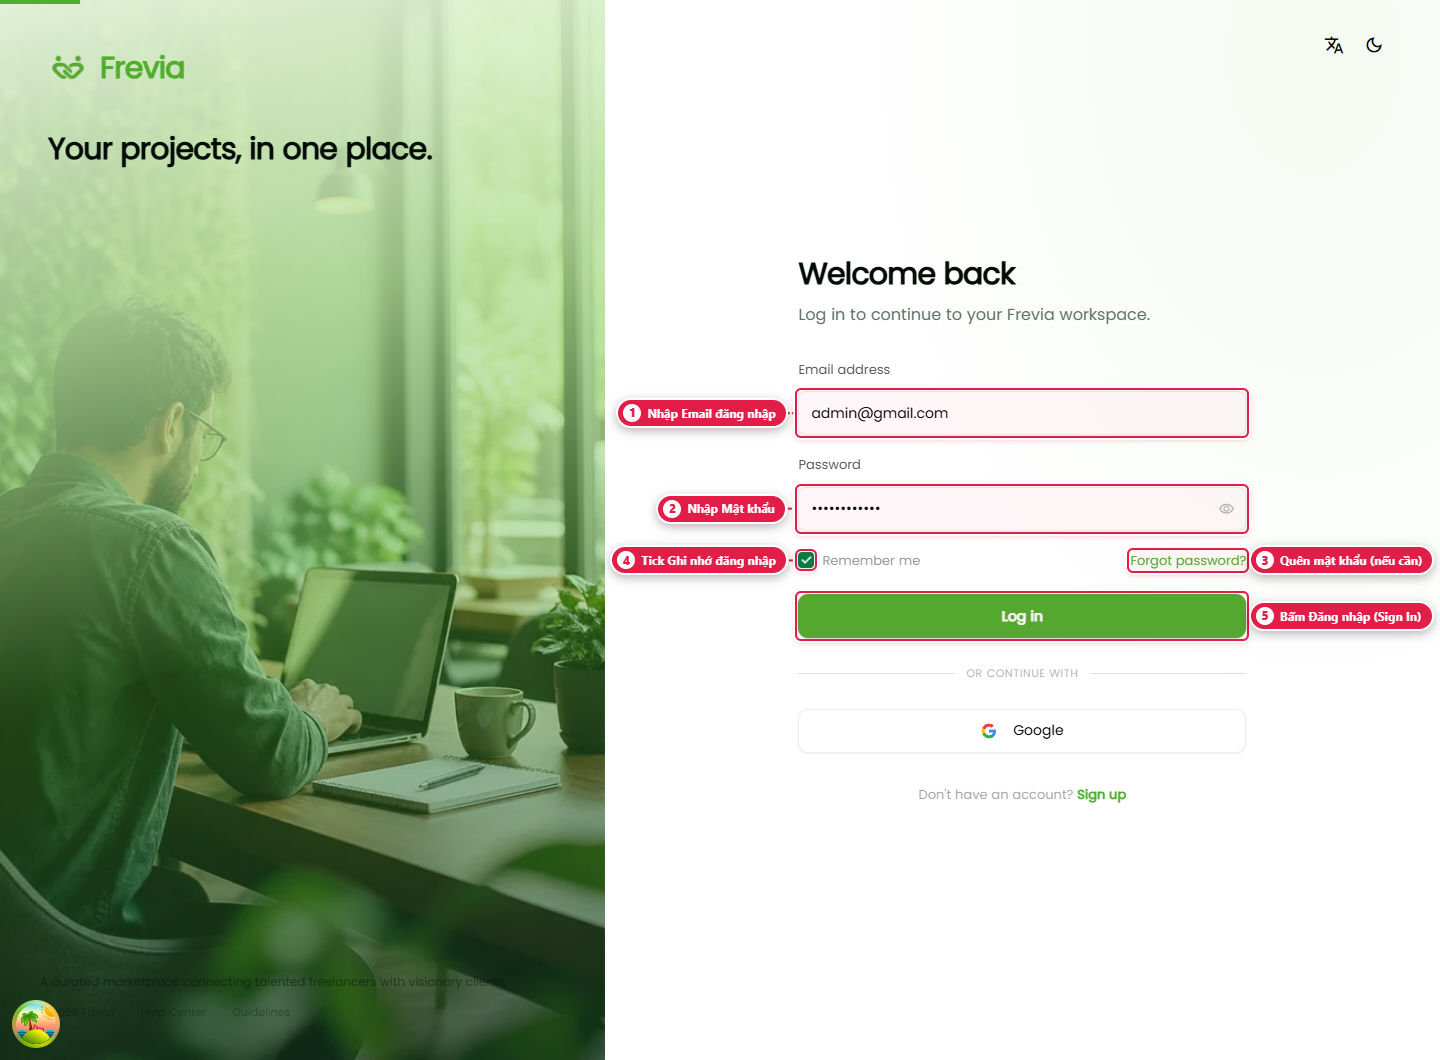
\includegraphics[width=0.90\textwidth]{images/auth/m02_02_login.png}
  \caption{User Login authentication screen at \texttt{/login}}
\end{figure}

\paragraph{Step-by-Step User Instructions:}
\begin{enumerate}[leftmargin=1.8em,itemsep=3pt]
  \item \rbadge{1} \textbf{Enter Registered Email (\textit{Email}):} Input the account email into the \textit{Email} field (e.g., \texttt{admin@gmail.com} or \texttt{freelancer@gmail.com}).
  \item \rbadge{2} \textbf{Enter Password (\textit{Password}):} Input the account password into the \textit{Password} field.
  \item \rbadge{3} \textbf{Toggle Persistent Session (\textit{Remember me}):} Check the \textit{Remember me} checkbox to extend session persistence across browser restarts.
  \item \rbadge{4} \textbf{Password Recovery Link (\textit{Forgot password?}):} If credentials have been forgotten, click the \textit{Forgot password?} link to initiate the recovery flow.
  \item \rbadge{5} \textbf{Click Sign In (\textit{Sign in}):} Click the blue \textbf{Sign in} button to authenticate.
\end{enumerate}

\paragraph{Expected Output \& Exception Handling:}
\begin{itemize}[leftmargin=1.5em,itemsep=2pt]
  \item \textbf{Success Scenario:} The backend verifies the \texttt{bcrypt} hash, creates an active \texttt{Session} entity recording client IP, User-Agent, and device metadata, sets secure \texttt{HttpOnly} cookies, and redirects the user:
    \begin{itemize}
      \item Accounts holding the \texttt{ADMIN} role are redirected to the administrator console at \texttt{/admin}.
      \item Freelancers and Clients are redirected to their tailored home dashboard.
    \end{itemize}
  \item \textbf{Exception Scenarios:}
    \begin{itemize}
      \item If credentials do not match, the application presents an error alert: \textit{"Invalid email or password"}.
      \item If the account is suspended, an alert states: \textit{"Your account has been suspended. Please contact support"}.
    \end{itemize}
\end{itemize}

% -----------------------------------------------------------------------------
\newpage
\subsubsection{M2.03 -- Single Sign-On via Google OAuth 2.0 (UC-03)}

\begin{itemize}[leftmargin=1.5em,itemsep=2pt]
  \item \textbf{Screen Name \& Route Path:} Social Sign-In Interface -- \texttt{/login}.
  \item \textbf{Target Actor:} Guest.
  \item \textbf{Preconditions:} The user possesses an active Google account.
\end{itemize}

\begin{figure}[H]
  \centering
  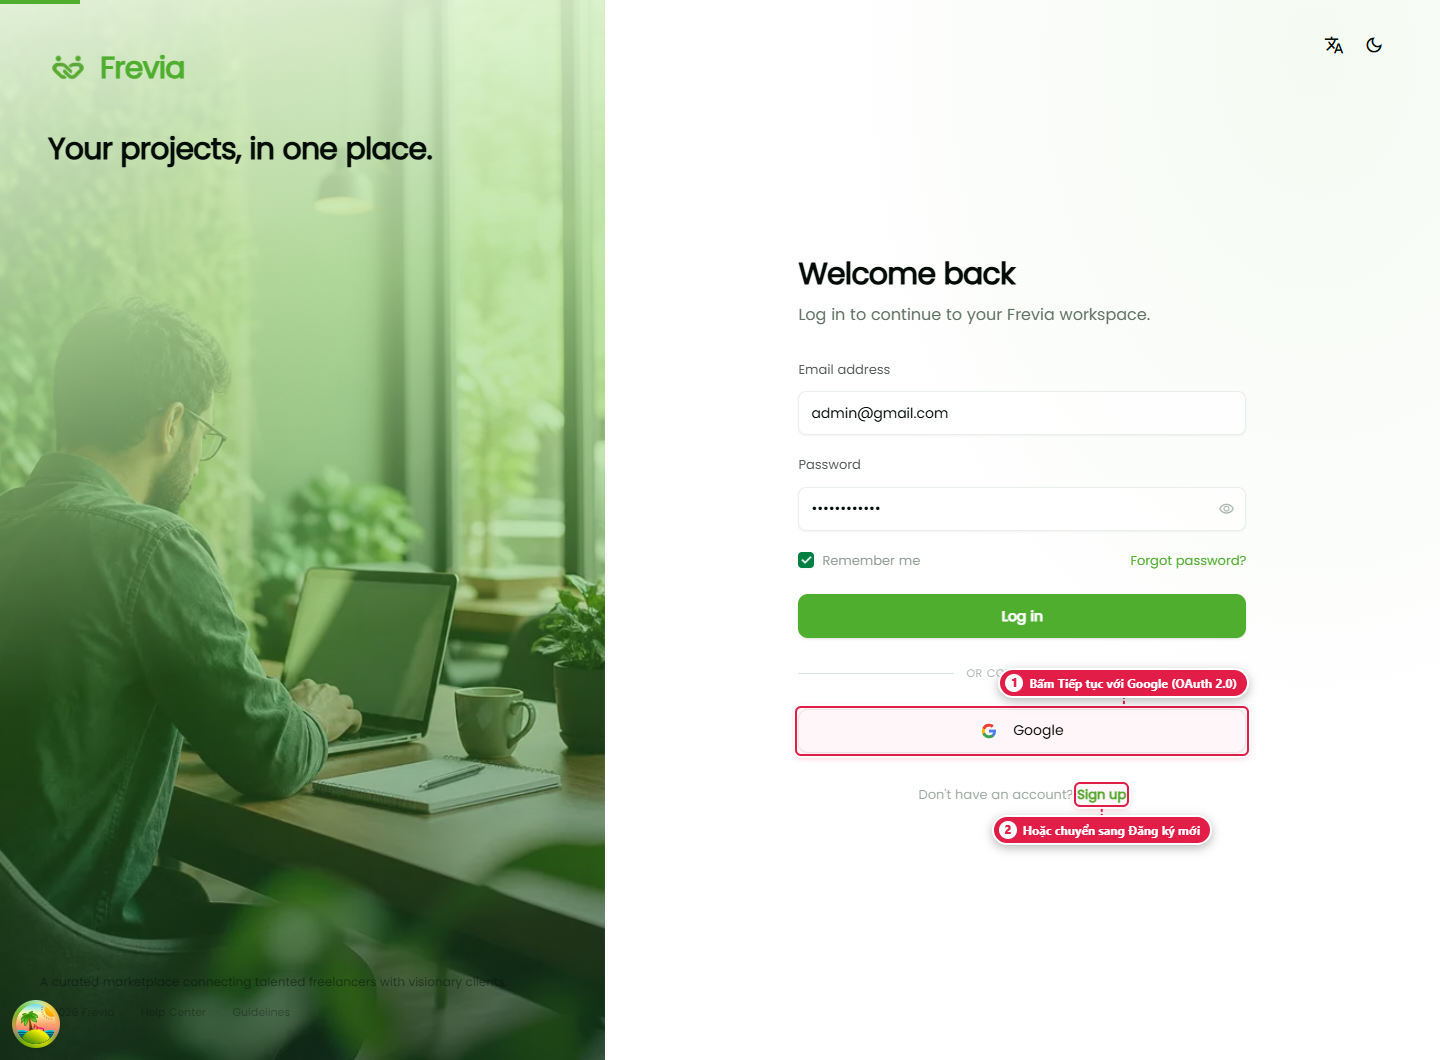
\includegraphics[width=0.90\textwidth]{images/auth/m02_03_google_oauth.png}
  \caption{Google OAuth 2.0 Single Sign-On button and registration link on the login screen}
\end{figure}

\paragraph{Step-by-Step User Instructions:}
\begin{enumerate}[leftmargin=1.8em,itemsep=3pt]
  \item \rbadge{1} \textbf{Click Google Sign-In Button (\textit{Continue with Google}):} Click the \textbf{Google} button beneath the divider to initiate federated authentication via the standard Google OAuth 2.0 consent flow.
  \item \rbadge{2} \textbf{Registration Navigation Link (\textit{Sign up}):} Alternatively, if the user does not possess an account, clicking \textit{Sign up} immediately routes to the registration view at \texttt{/register}.
\end{enumerate}

\paragraph{Expected Output \& Exception Handling:}
\begin{itemize}[leftmargin=1.5em,itemsep=2pt]
  \item \textbf{Success Scenario:} Google validates identity and redirects the browser back to \texttt{/api/auth/google/callback}. The backend links or provisions the user profile, sets authentication cookies, and signs the user in instantly.
  \item \textbf{Exception Scenarios:} If the user cancels the Google permission prompt, the callback redirects back to \texttt{/login} with a cancellation notification.
\end{itemize}

% -----------------------------------------------------------------------------
\newpage
\subsubsection{M2.04 -- Password Recovery \& Reset via Email OTP (UC-04)}

\begin{itemize}[leftmargin=1.5em,itemsep=2pt]
  \item \textbf{Screen Name \& Route Path:} Password Recovery Screen -- \texttt{/forgot-password}.
  \item \textbf{Target Actor:} Registered User who has forgotten their account password.
  \item \textbf{Preconditions:} The user knows the registered email address associated with their Frevia account.
\end{itemize}

\begin{figure}[H]
  \centering
  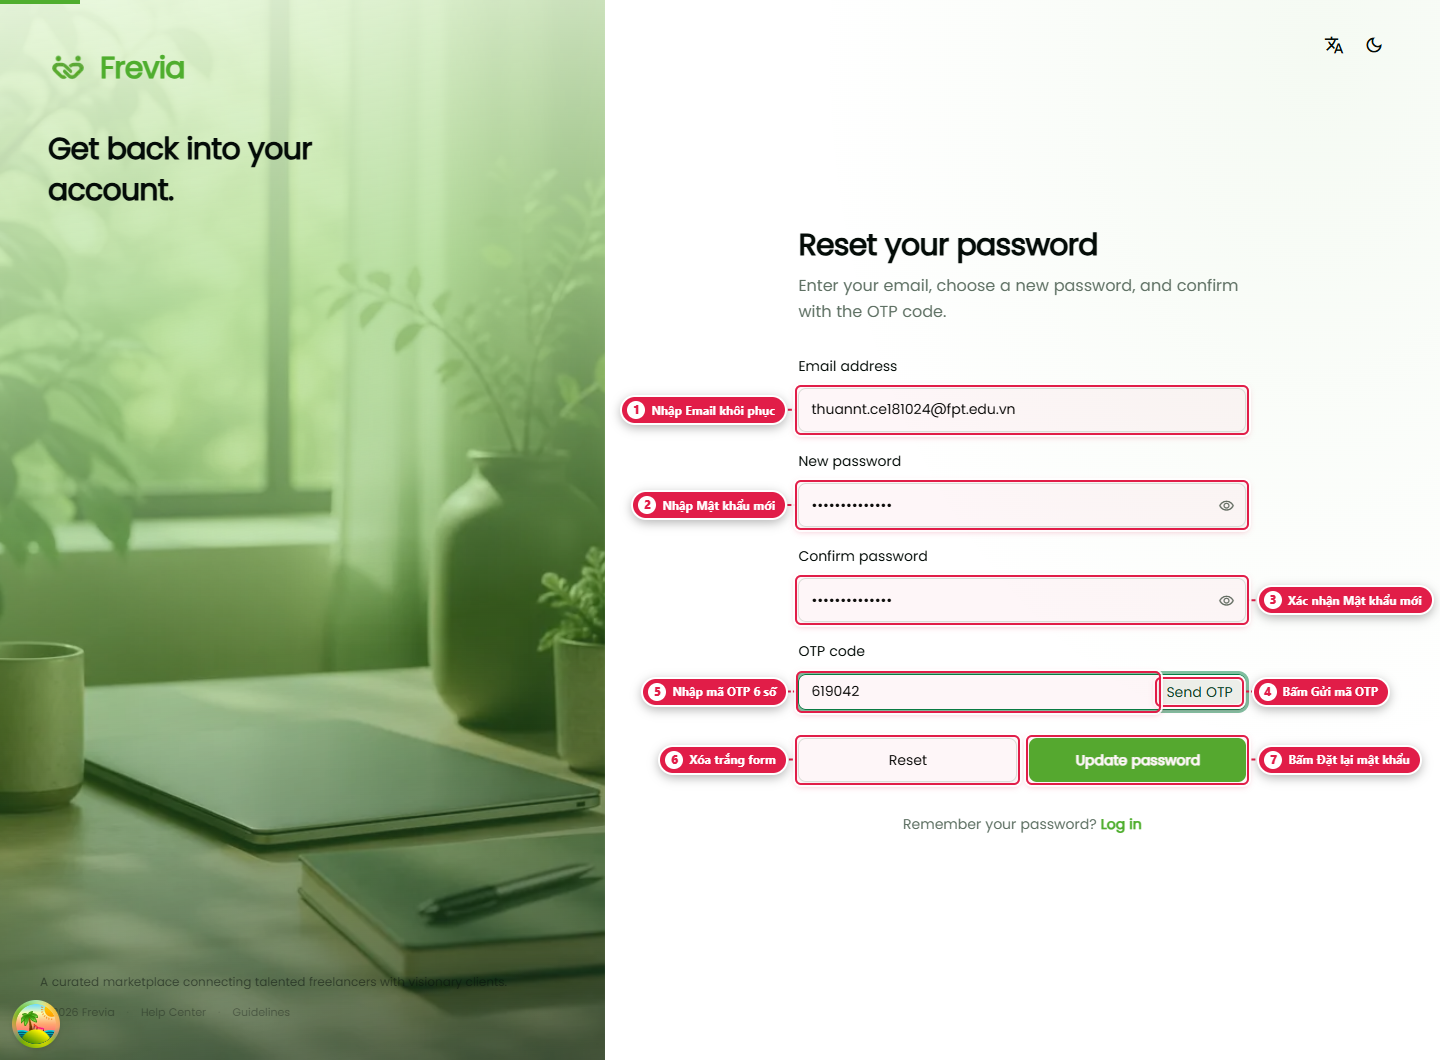
\includegraphics[width=0.90\textwidth]{images/auth/m02_04_forgot_password.png}
  \caption{Password recovery and OTP reset interface at \texttt{/forgot-password}}
\end{figure}

\paragraph{Step-by-Step User Instructions:}
\begin{enumerate}[leftmargin=1.8em,itemsep=3pt]
  \item \rbadge{1} \textbf{Enter Account Email (\textit{Email address}):} Type the registered email into the \textit{Email address} field.
  \item \rbadge{2} \textbf{Request Reset OTP (\textit{Send OTP}):} Click the blue \textbf{Send OTP} button to dispatch a reset code to the mailbox.
  \item \rbadge{3} \textbf{Enter Verification OTP (\textit{OTP code}):} Retrieve the 6-digit code from the received email and input it into the \textit{OTP code} field.
  \item \rbadge{4} \textbf{Enter New Password (\textit{New password}):} Type the replacement password (minimum 6 characters).
  \item \rbadge{5} \textbf{Confirm New Password (\textit{Confirm new password}):} Retype the new password to ensure consistency.
  \item \rbadge{6} \textbf{Submit Password Reset (\textit{Reset password}):} Click the blue \textbf{Reset password} button to commit changes.
  \item \rbadge{7} \textbf{Return to Sign In Link (\textit{Back to sign in}):} Click \textbf{Back to sign in} to return to \texttt{/login} without resetting.
\end{enumerate}

\paragraph{Expected Output \& Exception Handling:}
\begin{itemize}[leftmargin=1.5em,itemsep=2pt]
  \item \textbf{Success Scenario:} The server validates the OTP against Redis, re-hashes the new password with bcrypt, invalidates all existing active sessions for security, displays a confirmation toast, and redirects to \texttt{/login}.
  \item \textbf{Exception Scenarios:} If the OTP is invalid or expired, the submission is rejected with an explicit error alert.
\end{itemize}

% -----------------------------------------------------------------------------
\newpage
\subsubsection{M2.05 -- Active Login Session Monitoring \& Device Audit (UC-05.01)}

\begin{itemize}[leftmargin=1.5em,itemsep=2pt]
  \item \textbf{Screen Name \& Route Path:} Session Management Console -- \texttt{/sessions}.
  \item \textbf{Target Actor:} Authenticated User (Freelancer, Client, Expert, Admin).
  \item \textbf{Preconditions:} User is logged into the application with at least one active session record in the database.
\end{itemize}

\begin{figure}[H]
  \centering
  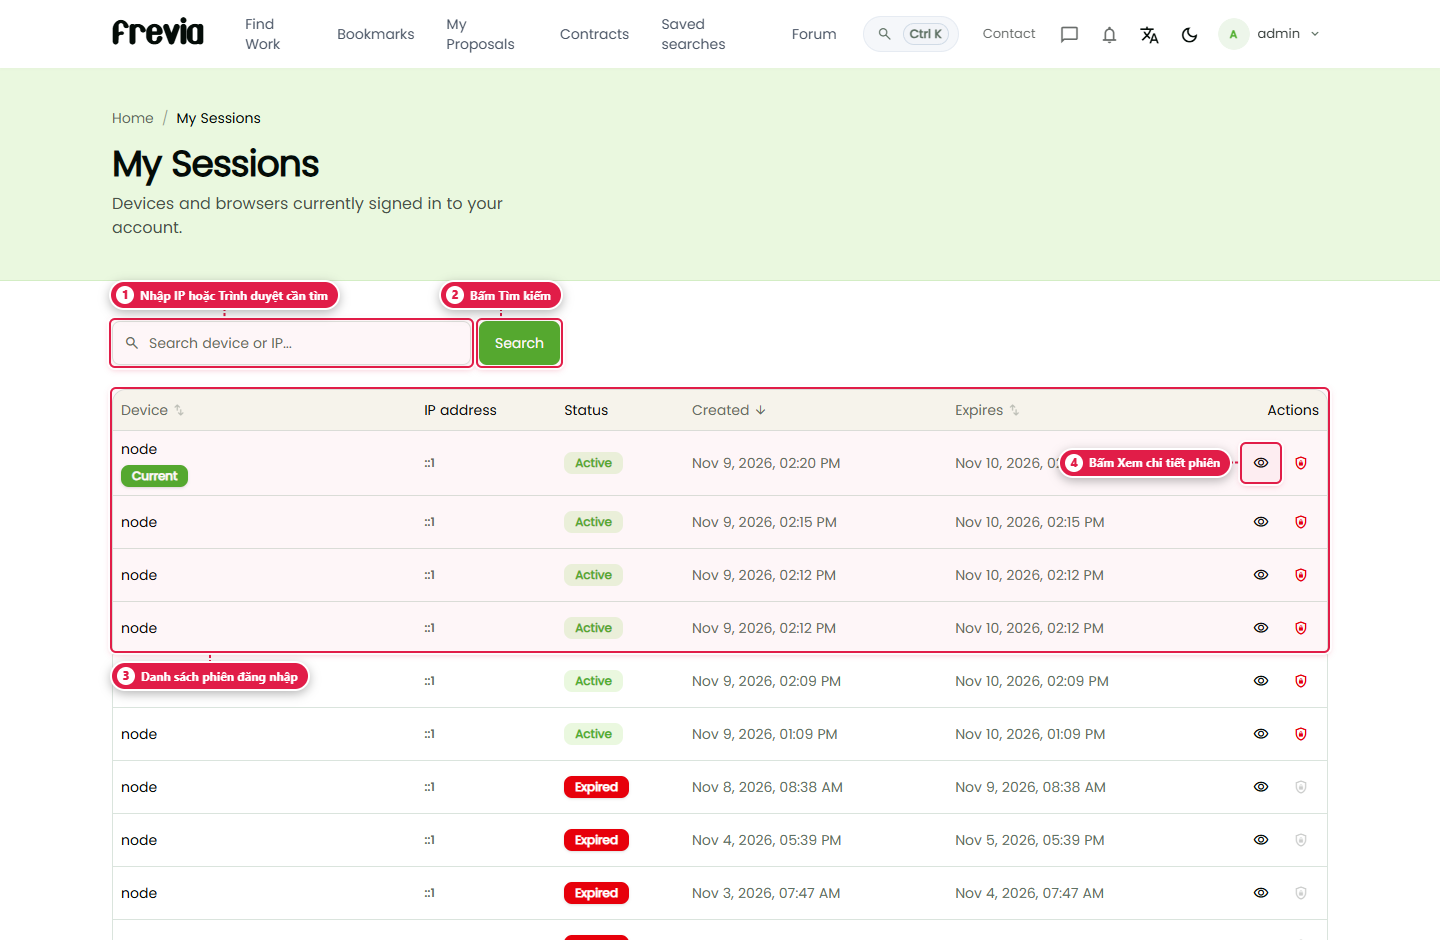
\includegraphics[width=0.90\textwidth]{images/auth/m02_05_sessions_list.png}
  \caption{Active login sessions audit table with search and filtering at \texttt{/sessions}}
\end{figure}

\paragraph{Step-by-Step User Instructions:}
\begin{enumerate}[leftmargin=1.8em,itemsep=3pt]
  \item Navigate to \url{http://localhost:3001/sessions} from the user settings menu.
  \item \rbadge{1} \textbf{Filter Sessions by Device / IP (\textit{Search input}):} Type a browser name, operating system, or IP address into the search box to dynamically filter listed records.
  \item \rbadge{2} \textbf{Inspect Active Session Records (\textit{Sessions table}):} Review session attributes across columns: \textit{Device / Browser} (detected User-Agent), \textit{IP Address}, \textit{Location}, \textit{Created} timestamp, and \textit{Status} (the active browser instance displays a blue \textbf{Current Session} badge).
  \item \rbadge{3} \textbf{Revoke Remote Session Button (\textit{Trash icon}):} Click the red trash icon on any remote session row to disconnect that specific device.
\end{enumerate}

\paragraph{Expected Output \& Exception Handling:}
\begin{itemize}[leftmargin=1.5em,itemsep=2pt]
  \item \textbf{Success Scenario:} The user gains full visibility over all authorized devices, identifying potential unauthorized account access.
\end{itemize}

% -----------------------------------------------------------------------------
\newpage
\subsubsection{M2.06 -- Remote Session Revocation \& Security Enforcement (UC-05.02)}

\begin{itemize}[leftmargin=1.5em,itemsep=2pt]
  \item \textbf{Screen Name \& Route Path:} Remote Session Termination Confirmation Dialog -- \texttt{/sessions}.
  \item \textbf{Target Actor:} Authenticated User.
  \item \textbf{Preconditions:} At least one non-current active session exists in the sessions table.
\end{itemize}

\begin{figure}[H]
  \centering
  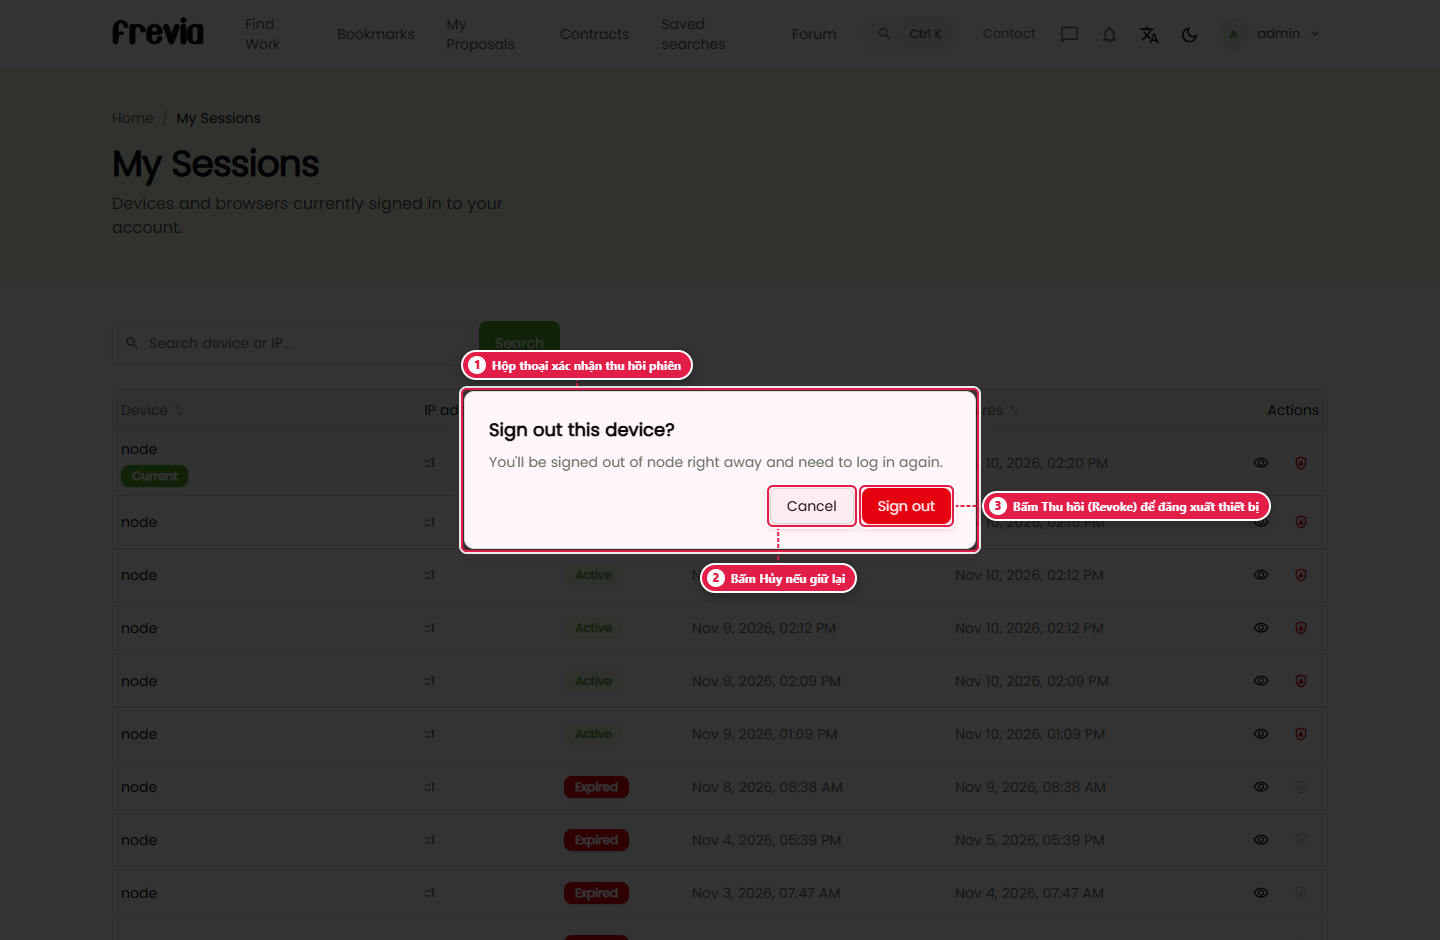
\includegraphics[width=0.90\textwidth]{images/auth/m02_06_revoke_session.png}
  \caption{Confirmation modal dialog for revoking a remote session at \texttt{/sessions}}
\end{figure}

\paragraph{Step-by-Step User Instructions:}
\begin{enumerate}[leftmargin=1.8em,itemsep=3pt]
  \item \rbadge{1} \textbf{Click Revoke Session Button:} In the session table, locate the target remote device row and click its red trash icon.
  \item \rbadge{2} \textbf{Read Revocation Warning (\textit{Dialog title \& description}):} An \texttt{AlertDialog} appears reading: \textit{"Revoke Session -- Are you sure you want to revoke this session? The device will be logged out immediately."}
  \item \rbadge{3} \textbf{Confirm Revocation Action (\textit{Revoke button}):} Click the red \textbf{Revoke} button to confirm immediate termination (or click \textit{Cancel} to dismiss the dialog without taking action).
\end{enumerate}

\paragraph{Expected Output \& Exception Handling:}
\begin{itemize}[leftmargin=1.5em,itemsep=2pt]
  \item \textbf{Success Scenario:} The backend invalidates the corresponding \texttt{RefreshToken} in PostgreSQL and purges the token from Redis. The targeted device will have its session rejected upon its subsequent API request and will be redirected to \texttt{/login}. A green toast confirms: \textit{"Session revoked successfully"}.
\end{itemize}

% -----------------------------------------------------------------------------
\newpage
\subsubsection{M2.07 -- Secure User Sign-Out \& Session Invalidation (UC-05.03)}

\begin{itemize}[leftmargin=1.5em,itemsep=2pt]
  \item \textbf{Screen Name \& Route Path:} Sidebar / Header Navigation across all portals.
  \item \textbf{Target Actor:} Authenticated User.
  \item \textbf{Preconditions:} User is currently logged into the system.
\end{itemize}

\begin{figure}[H]
  \centering
  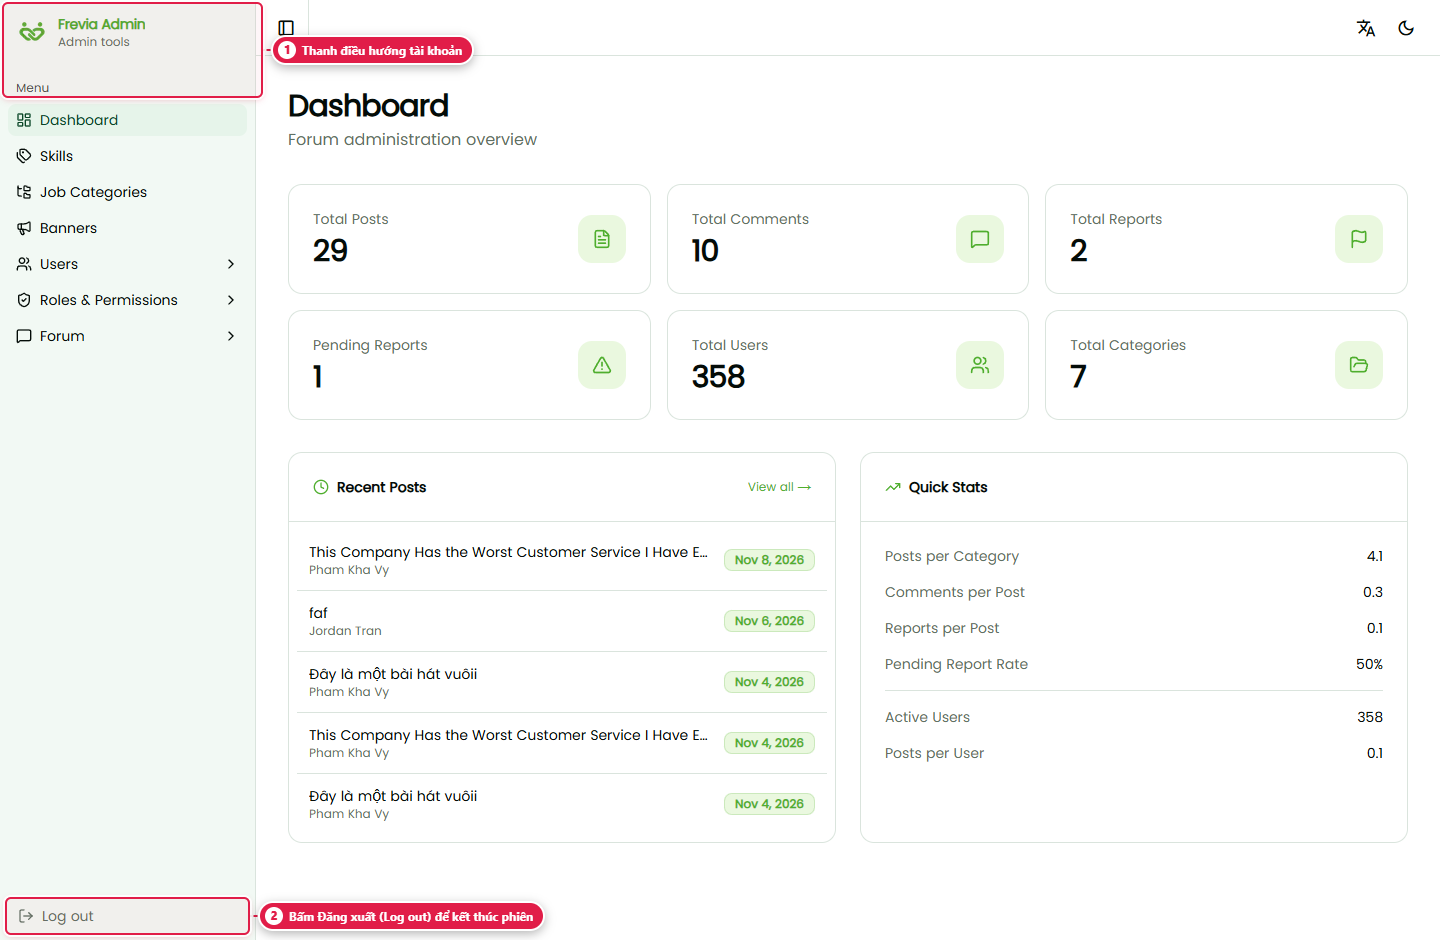
\includegraphics[width=0.90\textwidth]{images/auth/m02_07_logout.png}
  \caption{User identity card and sign-out button located in the application navigation bar}
\end{figure}

\paragraph{Step-by-Step User Instructions:}
\begin{enumerate}[leftmargin=1.8em,itemsep=3pt]
  \item \rbadge{1} \textbf{Inspect User Profile Summary:} In the lower left section of the sidebar navigation, observe the authenticated identity card showing Avatar, Full Name (\texttt{admin}), Email (\texttt{admin@gmail.com}), and role badge.
  \item \rbadge{2} \textbf{Click Sign Out Button (\textit{Logout icon}):} Click the red exit icon located on the right side of the identity card.
\end{enumerate}

\paragraph{Expected Output \& Exception Handling:}
\begin{itemize}[leftmargin=1.5em,itemsep=2pt]
  \item \textbf{Success Scenario:} The application dispatches an HTTP POST request to \texttt{/api/auth/logout}, expires client \texttt{HttpOnly} cookies, purges cached application state from TanStack Query, and redirects the browser cleanly to \texttt{/login}.
\end{itemize}
